\begin{figure}
    \centering
    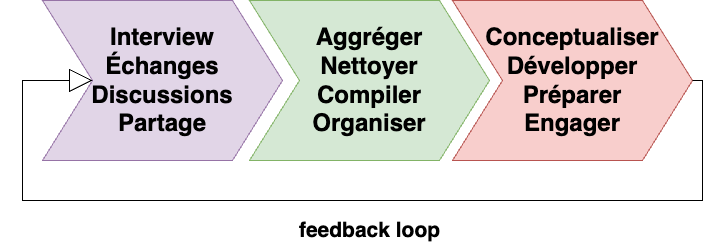
\includegraphics[width=0.75\linewidth]{images/Diagrams-Simplified framework chain Our approach.png}
    \caption{Notre approche simplifié}
    \label{fig:simplified-approach}
\end{figure}
Notre approche propose un cadre multi-axes pour aider les méta-organisations à évaluer l'impact via des méthodologies et outils basés sur les données. Nous présentons un cadre multi-étapes pour construire une solution de stockage de données orientée impact, allant de la collecte de preuves à l'analyse des indicateurs par des entretiens axés sur l'impact. Ce système permettrait aux méta-organisations de surveiller et d'évaluer régulièrement leur impact tout en engageant efficacement les partenaires internes et externes dans les changements. Nous avons identifié trois activités essentielles : la discussion, l'évaluation et la construction du système. Notre travail vise à transformer positivement le changement à l'intérieur des organisations et méta-organisations, avec des actions planifiées pour gérer la résistance et soutenir le changement via des feedbacks positifs. 